
%% ---------------------------------------------------------------------------
% This presentation is separated by sections and subsections

\begin{frame}[fragile]{\TeX 与 \LaTeX 的起源}
  \begin{columns}[T]
    \column{.8\textwidth}
    \begin{itemize}
      \item \TeX: $\tau\varepsilon\chi$ (\textipa{/'tEx/},
        \textipa{/'tEk/})
        \begin{itemize}
          \item 生成精美图书的排版系统
          \item 最初由 高德纳 (Donald E.~Knuth) 于 1978 年开发
          \item 最新版本为 \TeX\ 3.14159265
          \item 漂亮、美观、稳定、通用
          \item 尤其擅长数学公式排版
        \end{itemize}

        \vspace{2em}
      \item \LaTeX\ (\textipa{/'la:tEx/}, \textipa{/'leItEk/})
        \begin{itemize}
          \item Leslie Lamport 开发的一种 \TeX{} 格式
          \item 在 \TeX 的基础上提供宏包, 降低使用门槛
          \item 极其丰富的宏包,提供扩展功能
          \item 广泛用于学术界,期刊会议论文模板
        \end{itemize}
    \end{itemize}
    \column{.2\textwidth}
    % \vspace*{5mm}
    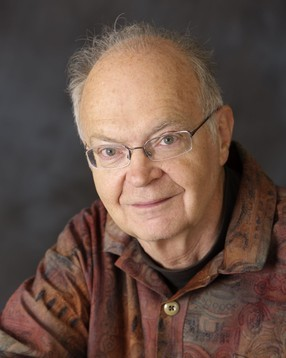
\includegraphics[width=\textwidth]{Knuth.jpg}

    % \vspace*{5mm}
    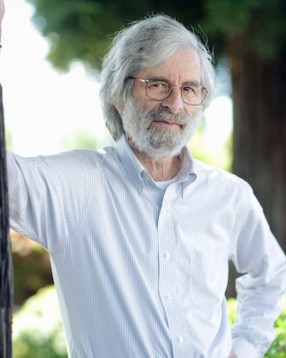
\includegraphics[width=\textwidth]{Lamport.jpg}

  \end{columns}
\end{frame}

\begin{frame}[fragile]{\LaTeX 的好处与坏处}
    \textbf{好处}
    \begin{itemize}
        \item 数学公式排版优雅 \quad $\mathcal{F}(\xi)=\int_{-\infty}^{\infty} f(x)\mathrm{e}^{-\mathrm{j}2\pi \xi x}\,\mathrm{d}x$
        \item 内容与格式分离
        \item 随心所欲的宏定义与自定义命令 \texttt{\textbackslash newcommand},\texttt{\textbackslash def}
    \end{itemize}

    \vspace{2em}
    \textbf{坏处}
    \begin{itemize}
        \item 得到易读的版本,需要编译
        \item 输入相对 Word 繁琐
        \item 非开箱即用。有时自行解决编辑器、宏包,甚至是编译错误。
    \end{itemize}

\end{frame}

